%Chapter 4

\chapter{Caso de estudio: diseño de interfaz}

Este capítulo presenta un estudio de caso que demuestra un proceso para diseñar funciones que trabajen juntas.

Introduce el módulo \texttt{turtle}, que te permite crear imágenes usando gráficos de tortuga. El módulo \texttt{turtle} está incluido en la mayoría de las instalaciones de Python, pero si estás ejecutando Python usando PythonAnywhere, no podrás ejecutar los ejemplos de turtle (al menos no podías cuando escribí esto).

Si ya has instalado Python en tu computadora, deberías poder ejecutar los ejemplos. De lo contrario, ahora es un buen momento para instalarlo. He publicado instrucciones en \url{http://tinyurl.com/thinkpython2e}.

Los ejemplos de código de este capítulo están disponibles en \url{https://thinkpython.com/code/polygon.py}.

\section{El módulo turtle}

Para verificar si tienes el módulo \texttt{turtle}, abre el intérprete de Python y escribe:

\begin{lstlisting}[language=Python]
>>> import turtle
>>> bob = turtle.Turtle()
\end{lstlisting}

Cuando ejecutes este código, debería crear una nueva ventana con una pequeña flecha que representa la tortuga. Cierra la ventana.

Crea un archivo llamado \texttt{mypolygon.py} y escribe el siguiente código:

\begin{lstlisting}[language=Python]
import turtle
bob = turtle.Turtle()
print(bob)
turtle.mainloop()
\end{lstlisting}

El módulo \texttt{turtle} (con `t' minúscula) proporciona una función llamada \texttt{Turtle} (con `T' mayúscula) que crea un objeto Turtle, que asignamos a una variable llamada \texttt{bob}. Imprimir \texttt{bob} muestra algo como:

\begin{lstlisting}[language=Python]
<turtle.Turtle object at 0xb7bfbf4c>
\end{lstlisting}

Esto significa que \texttt{bob} se refiere a un objeto de tipo \texttt{Turtle} definido en el módulo \texttt{turtle}.

\texttt{mainloop} le dice a la ventana que espere a que el usuario haga algo, aunque en este caso no hay mucho que hacer excepto cerrar la ventana.

Una vez que creas una Tortuga, puedes llamar a un \textbf{método} para moverla por la ventana. Un método es similar a una función, pero usa una sintaxis ligeramente diferente. Por ejemplo, para mover la tortuga hacia adelante:

\begin{lstlisting}[language=Python]
bob.fd(100)
\end{lstlisting}

El método \texttt{fd} está asociado con el objeto tortuga que llamamos \texttt{bob}. Llamar a un método es como hacer una petición: le estás pidiendo a \texttt{bob} que avance.

El argumento de \texttt{fd} es una distancia en píxeles, por lo que el tamaño real depende de tu pantalla.

Otros métodos que puedes llamar en una Tortuga son \texttt{bk} para mover hacia atrás, \texttt{lt} para girar a la izquierda y \texttt{rt} para girar a la derecha. El argumento para \texttt{lt} y \texttt{rt} es un ángulo en grados.

Además, cada Tortuga sostiene un lápiz, que puede estar arriba o abajo; si el lápiz está abajo, la Tortuga deja un rastro cuando se mueve. Los métodos \texttt{pu} y \texttt{pd} significan ``lápiz arriba'' y ``lápiz abajo''.

Para dibujar un ángulo recto, agrega estas líneas al programa (después de crear \texttt{bob} y antes de llamar a \texttt{mainloop}):

\begin{lstlisting}[language=Python]
bob.fd(100)
bob.lt(90)
bob.fd(100)
\end{lstlisting}

Cuando ejecutes este programa, deberías ver a \texttt{bob} moverse hacia el este y luego hacia el norte, dejando dos segmentos de línea atrás.

Ahora modifica el programa para dibujar un cuadrado. ¡No continúes hasta que lo hayas hecho funcionar!

\section{Repetición simple}

Es probable que hayas escrito algo como esto:

\begin{lstlisting}[language=Python]
bob.fd(100)
bob.lt(90)

bob.fd(100)
bob.lt(90)

bob.fd(100)
bob.lt(90)

bob.fd(100)
\end{lstlisting}

Podemos hacer lo mismo de forma más concisa con una sentencia \texttt{for}. Agrega este ejemplo a \texttt{mypolygon.py} y ejecútalo nuevamente:

\begin{lstlisting}[language=Python]
for i in range(4):
    print('Hello!')
\end{lstlisting}

Deberías ver algo como esto:

\begin{lstlisting}[language=Python]
Hello!
Hello!
Hello!
Hello!
\end{lstlisting}

Este es el uso más simple de la sentencia \texttt{for}; veremos más ejemplos más adelante. Pero esto debería ser suficiente para permitirte reescribir tu programa de dibujo de cuadrados. No continúes hasta que lo hayas implementado.

Aquí hay una sentencia \texttt{for} que dibuja un cuadrado:

\begin{lstlisting}[language=Python]
for i in range(4):
    bob.fd(100)
    bob.lt(90)
\end{lstlisting}

La sintaxis de una sentencia \texttt{for} es similar a una definición de función:
\begin{itemize}
\item Tiene un encabezado que termina con dos puntos
\item Un cuerpo indentado (normalmente 4 espacios)
\item Puede contener cualquier número de declaraciones en el cuerpo
\end{itemize}

Una sentencia \texttt{for} también se denomina \textbf{bucle} porque el flujo de ejecución:
\begin{enumerate}
\item Recorre el cuerpo
\item Vuelve al principio
\item Repite el proceso hasta completar las iteraciones
\end{enumerate}

En este caso particular:
\begin{itemize}
\item El bucle se ejecuta exactamente 4 veces (\texttt{range(4)})
\item Cada iteración mueve la tortuga y gira 90 grados
\item La última iteración deja a \texttt{bob} en la posición inicial
\end{itemize}

Esta implementación tiene dos ventajas clave respecto a la versión anterior:
\begin{itemize}
\item \textbf{Consistencia}: Realiza la misma acción en cada iteración
\item \textbf{Simplicidad}: Elimina código repetido haciendo el programa más corto y legible
\end{itemize}

El pequeño giro extra al final no afecta el resultado final pero simplifica considerablemente la lógica del programa.

\section{Ejercicios}

La siguiente es una serie de ejercicios utilizando el módulo turtle. Están diseñados para ser divertidos, pero también tienen un propósito educativo. Mientras trabajas en ellos, piensa en qué concepto ilustra cada uno.

\begin{enumerate}
\item \textbf{Función square}: Escribe una función llamada \texttt{square} que tome un parámetro \texttt{t}, que es una tortuga. Debe usar la tortuga para dibujar un cuadrado. Escribe una llamada a función que pase \texttt{bob} como argumento a \texttt{square} y ejecuta el programa nuevamente.



\item \textbf{Parámetro length}: Añade otro parámetro llamado \texttt{length} a \texttt{square}. Modifica el cuerpo para que el largo de los lados sea \texttt{length}, y modifica la llamada a función para proporcionar este segundo argumento. Prueba tu programa con diferentes valores para \texttt{length}.



\item \textbf{Función polygon}: Haz una copia de \texttt{square} y cámbiale el nombre a \texttt{polygon}. Añade otro parámetro llamado \texttt{n} y modifica el cuerpo para que dibuje un polígono regular de \texttt{n} lados.



\item \textbf{Función circle}: Escribe una función llamada \texttt{circle} que tome una tortuga \texttt{t} y un radio \texttt{r} como parámetros, y que dibuje un círculo aproximado llamando a \texttt{polygon} con los valores apropiados.



\item \textbf{Función arc}: Haz una versión más general de \texttt{circle} llamada \texttt{arc} que tome un parámetro adicional \texttt{angle}, que determina qué fracción de círculo dibujar. \texttt{angle} está en grados, así que cuando \texttt{angle=360}, \texttt{arc} debe dibujar un círculo completo.


\end{enumerate}

\textbf{Consejos para los ejercicios}:
\begin{itemize}
\item Recuerda que cada ejercicio parte del anterior - construye sobre lo que ya tienes
\item El código debe estar en un archivo de script (con extensión .py), no en el intérprete interactivo
\item Considera usar nombres descriptivos para variables y parámetros
\item Prueba cada función con diferentes valores para asegurarte que funciona correctamente
\item Si el programa falla, los mensajes de error suelen indicar dónde está el problema
\end{itemize}

Al completar estos ejercicios, habrás creado un pequeño conjunto de funciones de dibujo geométrico que podrás reutilizar en proyectos futuros. La clave está en entender cómo cada generalización amplía las posibilidades de lo que puedes dibujar con patrones simples.

\section{Encapsulación}

El primer ejercicio te pide que coloques tu código para dibujar un cuadrado en una definición de función y luego llames a esa función, pasando la tortuga como parámetro. Aquí hay una solución:

\begin{lstlisting}[language=Python]
def square(t):
    for i in range(4):
        t.fd(100)
        t.lt(90)

square(bob)
\end{lstlisting}

Las declaraciones más internas, \texttt{fd} y \texttt{lt}, tienen doble sangría para mostrar que están dentro del bucle \texttt{for}, que a su vez está dentro de la definición de función. La siguiente línea, \texttt{square(bob)}, está alineada con el margen izquierdo, lo que indica el final tanto del bucle \texttt{for} como de la definición de función.

Dentro de la función, \texttt{t} se refiere a la misma tortuga \texttt{bob}, por lo que \texttt{t.lt(90)} tiene el mismo efecto que \texttt{bob.lt(90)}. En ese caso, ¿por qué no llamar al parámetro \texttt{bob}? La idea es que \texttt{t} puede ser cualquier tortuga, no solo \texttt{bob}, por lo que podrías crear una segunda tortuga y pasarla como argumento a \texttt{square}:

\begin{lstlisting}[language=Python]
alice = turtle.Turtle()
square(alice)
\end{lstlisting}

Envolver un fragmento de código en una función se llama \textbf{encapsulación}. Uno de los beneficios de la encapsulación es que asocia un nombre al código, lo que sirve como una especie de documentación. Otra ventaja es que si reutilizas el código, es más conciso llamar a una función dos veces que copiar y pegar el cuerpo.

\section{Generalización}

El siguiente paso es agregar un parámetro \texttt{length} a \texttt{square}. Aquí hay una solución:

\begin{lstlisting}[language=Python]
def square(t, length):
    for i in range(4):
        t.fd(length)
        t.lt(90)

square(bob, 100)
\end{lstlisting}

Agregar un parámetro a una función se llama \textbf{generalización} porque hace que la función sea más general: en la versión anterior, el cuadrado siempre tenía el mismo tamaño; en esta versión puede ser de cualquier tamaño.

El siguiente paso también es una generalización. En lugar de dibujar cuadrados, \texttt{polygon} dibuja polígonos regulares con cualquier número de lados. Aquí hay una solución:

\begin{lstlisting}[language=Python]
def polygon(t, n, length):
    angle = 360 / n
    for i in range(n):
        t.fd(length)
        t.lt(angle)

polygon(bob, 7, 70)  # Dibuja un heptágono
\end{lstlisting}

Este ejemplo dibuja un polígono de 7 lados con longitud de lado 70.

Si estás usando Python 2, el valor de \texttt{angle} podría ser incorrecto debido a la división de enteros. Una solución simple es calcular \texttt{angle = 360.0 / n}. Como el numerador es un número de punto flotante, el resultado también lo será.

Cuando una función tiene varios parámetros numéricos, es fácil olvidar qué son o en qué orden deben ir. En ese caso, a menudo es una buena idea incluir los nombres de los parámetros en la lista de argumentos:

\begin{lstlisting}[language=Python]
polygon(bob, n=7, length=70)
\end{lstlisting}

Estos se llaman \textbf{argumentos de palabras clave} porque incluyen los nombres de los parámetros como "palabras clave" (no confundir con las palabras clave de Python como \texttt{while} y \texttt{def}).

Esta sintaxis hace que el programa sea más legible. También es un recordatorio de cómo funcionan los argumentos y parámetros: cuando llamas a una función, los argumentos se asignan a los parámetros.

\section{Diseño de interfaces}

El siguiente paso es escribir \texttt{circle}, que toma un radio \texttt{r} como parámetro. Aquí hay una solución simple que usa \texttt{polygon} para dibujar un polígono de 50 lados:

\begin{lstlisting}[language=Python]
import math

def circle(t, r):
    circumference = 2 * math.pi * r
    n = 50
    length = circumference / n
    polygon(t, n, length)
\end{lstlisting}

La primera línea calcula la circunferencia de un círculo con radio \texttt{r} usando la fórmula $2\pi r$. Como usamos \texttt{math.pi}, necesitamos importar el módulo \texttt{math}. Por convención, las sentencias \texttt{import} suelen estar al comienzo del script.

\texttt{n} es el número de segmentos de línea en nuestra aproximación de un círculo, por lo que \texttt{length} es la longitud de cada segmento. Así, \texttt{polygon} dibuja un polígono de 50 lados que aproxima un círculo con radio \texttt{r}.

Esta solución tiene una limitación importante: \texttt{n} es una constante, lo que significa que para círculos muy grandes, los segmentos de línea son demasiado largos, y para círculos pequeños, perdemos tiempo dibujando segmentos muy pequeños. Una solución sería generalizar la función tomando \texttt{n} como parámetro, pero esto haría menos limpia la interfaz.

La \textbf{interfaz} de una función es un resumen de cómo se usa: ¿qué parámetros necesita? ¿Qué hace? ¿Qué valor retorna? Una interfaz es "limpia" si permite al usuario hacer lo que necesita sin lidiar con detalles innecesarios.

En este ejemplo, \texttt{r} pertenece a la interfaz porque especifica el círculo a dibujar. \texttt{n} es menos apropiado porque pertenece a los detalles de \textit{cómo} se debe renderizar el círculo.


En lugar de ensuciar la interfaz, podemos elegir un valor apropiado de \texttt{n} en función de la circunferencia:

\begin{lstlisting}[language=Python]
def circle(t, r):
    circumference = 2 * math.pi * r
    n = int(circumference / 3) + 3
    length = circumference / n
    polygon(t, n, length)
\end{lstlisting}

Ahora el número de segmentos es un entero cercano a \texttt{circumference/3}, por lo que cada segmento tendrá aproximadamente 3 píxeles de largo, lo suficientemente pequeño para que los círculos se vean bien, pero lo suficientemente grande como para ser eficiente y aceptable para círculos de cualquier tamaño.

Agregar 3 a \texttt{n} garantiza que el polígono tenga al menos 3 lados.

\section{Refactorización}

Cuando escribí \texttt{circle}, pude reutilizar \texttt{polygon} porque un polígono de muchos lados es una buena aproximación de un círculo. Pero con \texttt{arc} no somos tan afortunados; no podemos usar \texttt{polygon} o \texttt{circle} para dibujar un arco.


Una alternativa es comenzar con una copia de \texttt{polygon} y transformarla en \texttt{arc}. El resultado podría verse así:

\begin{lstlisting}[language=Python]
def arc(t, r, angle):
    arc_length = 2 * math.pi * r * angle / 360
    n = int(arc_length / 3) + 1
    step_length = arc_length / n
    step_angle = angle / n
    
    for i in range(n):
        t.fd(step_length)
        t.lt(step_angle)
\end{lstlisting}

La segunda mitad de esta función se parece a \texttt{polygon}, pero no podemos reutilizar \texttt{polygon} sin cambiar la interfaz. Podríamos generalizar \texttt{polygon} para tomar un ángulo como tercer argumento, pero entonces \texttt{polygon} ya no sería el nombre apropiado. En su lugar, llamemos a esta función más general \texttt{polyline}:

\begin{lstlisting}[language=Python]
def polyline(t, n, length, angle):
    for i in range(n):
        t.fd(length)
        t.lt(angle)
\end{lstlisting}

Ahora podemos reescribir \texttt{polygon} y \texttt{arc} para usar \texttt{polyline}:

\begin{lstlisting}[language=Python]
def polygon(t, n, length):
    angle = 360.0 / n
    polyline(t, n, length, angle)

def arc(t, r, angle):
    arc_length = 2 * math.pi * r * angle / 360
    n = int(arc_length / 3) + 1
    step_length = arc_length / n
    step_angle = float(angle) / n
    polyline(t, n, step_length, step_angle)
\end{lstlisting}

Finalmente, podemos reescribir \texttt{circle} para usar \texttt{arc}:

\begin{lstlisting}[language=Python]
def circle(t, r):
    arc(t, r, 360)
\end{lstlisting}

Este proceso - reorganizar un programa para mejorar las interfaces y facilitar la reutilización del código - se llama \textbf{refactorización}. En este caso, notamos que había código similar en \texttt{arc} y \texttt{polygon}, así que lo "factorizamos" en \texttt{polyline}.

Si hubiéramos planeado desde el principio, podríamos haber escrito \texttt{polyline} primero y evitado la refactorización, pero a menudo no se sabe lo suficiente al comienzo de un proyecto para diseñar todas las interfaces. Cuando empiezas a codificar, comprendes mejor el problema. A veces refactorizar es una señal de que has aprendido algo.


\section{Un plan de desarrollo}

Un \textbf{plan de desarrollo} es un proceso para escribir programas. El proceso que utilizamos en este estudio de caso es "encapsulación y generalización". Los pasos de este proceso son:

\begin{enumerate}
    \item Comienza escribiendo un programa pequeño sin definiciones de funciones.
    \item Una vez que el programa funcione, identifica una parte coherente del mismo, encapsula esa parte en una función y asígnale un nombre.
    \item Generaliza la función añadiendo los parámetros adecuados.
    \item Repite los pasos 1-3 hasta que tengas un conjunto de funciones que funcionen. Copia y pega el código funcional para evitar volver a escribirlo (y volver a depurarlo).
    \item Busca oportunidades para mejorar el programa mediante refactorización. Por ejemplo, si tienes código similar en varios lugares, considera factorizarlo en una función general adecuada.
\end{enumerate}

Este proceso tiene algunos inconvenientes (veremos alternativas más adelante), pero puede ser útil si no sabes de antemano cómo dividir el programa en funciones. Este enfoque te permite diseñar sobre la marcha.

\section{Documentación con docstrings}

Un \textbf{docstring} es una cadena de texto al comienzo de una función que explica su interfaz ("doc" es una abreviatura de "documentación"). Aquí tienes un ejemplo:

\begin{lstlisting}[language=Python]
def polyline(t, n, length, angle):
    """Dibuja n segmentos de línea con la longitud y
    ángulo (en grados) dados entre ellos. t es una tortuga.
    """
    for i in range(n):
        t.fd(length)
        t.lt(angle)
\end{lstlisting}

Por convención, todos los docstrings son cadenas entre comillas triples, también conocidas como cadenas multilínea porque las comillas triples permiten que la cadena abarque más de una línea.

Es conciso, pero contiene la información esencial que alguien necesitaría para usar esta función. Explica de manera breve lo que hace la función (sin entrar en detalles sobre cómo lo hace). También explica el efecto de cada parámetro en el comportamiento de la función y el tipo que debe tener cada parámetro (si no es obvio).

Escribir este tipo de documentación es una parte importante del diseño de interfaces. Una interfaz bien diseñada debe ser sencilla de explicar; si te cuesta explicar una de tus funciones, quizás la interfaz podría mejorarse.

\section{Depuración}

Una interfaz es como un contrato entre una función y quien la llama. Quien llama acepta proporcionar ciertos parámetros, y la función acepta realizar cierto trabajo.

Por ejemplo, \texttt{polyline} requiere cuatro argumentos: \texttt{t} debe ser una tortuga; \texttt{n} debe ser un entero; \texttt{length} debe ser un número positivo; y \texttt{angle} debe ser un número, que se entiende que está en grados.

Estos requisitos se llaman \textbf{precondiciones} porque se supone que deben ser verdaderos antes de que la función comience a ejecutarse. Por el contrario, las condiciones al final de la función se llaman \textbf{postcondiciones}. Las postcondiciones incluyen el efecto previsto de la función (como dibujar segmentos de línea) y cualquier efecto secundario (como mover la tortuga o realizar otros cambios).

Las precondiciones son responsabilidad de quien llama a la función. Si quien llama viola una precondición (¡correctamente documentada!) y la función no funciona correctamente, el error está en quien llama, no en la función.

Si las precondiciones se cumplen y las postcondiciones no, el error está en la función. Si tus precondiciones y postcondiciones son claras, pueden ayudarte en la depuración.

\section{Glosario}

\begin{itemize}
    \item \textbf{método}: Una función asociada a un objeto y llamada usando notación de punto.
    \item \textbf{bucle}: Parte de un programa que puede ejecutarse repetidamente.
    \item \textbf{encapsulación}: Proceso de transformar una secuencia de sentencias en una definición de función.
    \item \textbf{generalización}: Proceso de reemplazar algo innecesariamente específico (como un número) con algo más general (como una variable o parámetro).
    \item \textbf{argumento de palabra clave}: Argumento que incluye el nombre del parámetro como "palabra clave".
    \item \textbf{interfaz}: Descripción de cómo usar una función, incluyendo el nombre y descripciones de los argumentos y el valor de retorno.
    \item \textbf{refactorización}: Proceso de modificar un programa funcional para mejorar las interfaces de las funciones y otras cualidades del código.
    \item \textbf{plan de desarrollo}: Proceso para escribir programas.
    \item        
        \begin{figure}[h]
        \centering
        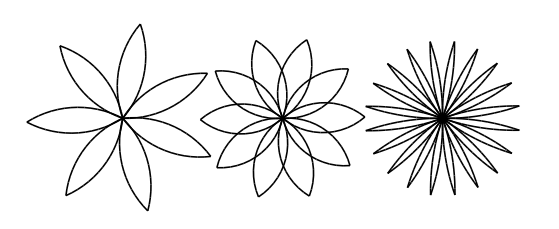
\includegraphics[width=0.5\textwidth]{./images/chapter_4_1.png}
        \caption{Flores Turtle.}
        \label{fig:4_1}
        \end{figure}
    \item        
        \begin{figure}[h]
        \centering
        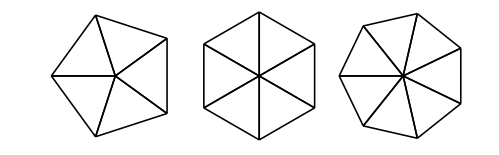
\includegraphics[width=0.5\textwidth]{./images/chapter_4_2.png}
        \caption{Turtle Pies.}
        \label{fig:4_2}
        \end{figure}
    \item \textbf{docstring}: Cadena que aparece al principio de una definición de función para documentar su interfaz.
    \item \textbf{precondición}: Requisito que debe cumplir quien llama a una función antes de que esta comience.
    \item \textbf{postcondición}: Requisito que debe cumplir la función antes de finalizar.
\end{itemize}

\section{Ejercicios}

\begin{enumerate}
    \item \textbf{Ejercicio 4.1}: Descarga el código de este capítulo desde \url{https://thinkpython.com/code/polygon.py}.
    \begin{enumerate}
        \item Dibuja un diagrama de pila que muestre el estado del programa mientras ejecuta \texttt{circle(bob, radius)}. Puedes hacer los cálculos a mano o añadir sentencias \texttt{print} al código.
        \item La versión de \texttt{arc} en la Sección 4.7 no es muy precisa porque la aproximación lineal del círculo siempre está fuera del círculo verdadero. Como resultado, la tortuga termina unos píxeles lejos del destino correcto. Mi solución muestra una manera de reducir el efecto de este error. Lee el código y comprueba si tiene sentido para ti. Si dibujas un diagrama, podrías ver cómo funciona.
    \end{enumerate}
    
    \item \textbf{Ejercicio 4.2}: Escribe un conjunto de funciones adecuadamente generales que puedan dibujar flores como en la Figura 4.1. \\
    Solución: \url{https://thinkpython.com/code/flower.py}, también requiere \url{https://thinkpython.com/code/polygon.py}.
    
    \item \textbf{Ejercicio 4.3}: Escribe un conjunto de funciones adecuadamente generales que puedan dibujar formas como en la Figura 4.2. \\
    Solución: \url{https://thinkpython.com/code/pie.py}.
    
    \item \textbf{Ejercicio 4.4}: Las letras del alfabeto pueden construirse a partir de un número moderado de elementos básicos, como líneas verticales y horizontales y algunas curvas. Diseña un alfabeto que pueda dibujarse con un número mínimo de elementos básicos y luego escribe funciones que dibujen las letras. \\
    Debes escribir una función para cada letra, con nombres como \texttt{draw\_a}, \texttt{draw\_b}, etc., y colocar tus funciones en un archivo llamado \texttt{letters.py}. Puedes descargar una "máquina de escribir de tortuga" desde \url{https://thinkpython.com/code/typewriter.py} para ayudarte a probar tu código. \\
    Solución: \url{https://thinkpython.com/code/letters.py}; también requiere \url{https://thinkpython.com/code/polygon.py}.
    
    \item \textbf{Ejercicio 4.5}: Lee sobre espirales en \url{http://en.wikipedia.org/wiki/Spiral}; luego escribe un programa que dibuje una espiral de Arquímedes (o algún otro tipo). \\
    Solución: \url{https://thinkpython.com/code/spiral.py}.
\end{enumerate}

